\documentclass[11pt,a4paper]{article}
\usepackage{fontspec}
\setmainfont{TeX Gyre Pagella}
\newfontfamily\headfont{Inter}[UprightFont=*-ExtraBold,BoldFont=*-ExtraBold,Extension=.otf,Path=/usr/share/fonts/opentype/inter/]
\usepackage[a4paper,margin=2.3cm]{geometry}
\usepackage{graphicx,booktabs,float,caption,array,xcolor,longtable}
\usepackage{xurl}
\usepackage[hidelinks]{hyperref}
\usepackage{titlesec}
\usepackage[round]{natbib}
\usepackage{setspace}
\setstretch{1.05}
\renewcommand{\topfraction}{0.9}
\renewcommand{\bottomfraction}{0.8}
\renewcommand{\textfraction}{0.1}
\renewcommand{\floatpagefraction}{0.75}
\setlength{\parindent}{0pt}
\setlength{\parskip}{0.55em}
\titleformat{\section}{\headfont\Large}{\thesection}{0.8em}{}
\titleformat{\subsection}{\headfont\large}{\thesubsection}{0.8em}{}
\captionsetup{font=small,labelfont=bf}
\urlstyle{same}
\hypersetup{pdftitle={London's Buried Rivers},pdfauthor={Tristan Hotham}}

\begin{document}
\begin{center}
{\Large\bfseries London's Buried Rivers\par}
\vspace{0.4em}
{\large Open and culverted waterways in OpenStreetMap,\\and the lost rivers beneath the city\par}
\vspace{1.2em}
{\large Tristan Hotham\par}
\vspace{0.3em}
{\small Independent researcher\\
ORCID: 0000-0003-4931-9349\\
DOI: https://doi.org/10.5281/zenodo.23873535\par}
\vspace{0.8em}
2026
\end{center}

\begin{quote}
\small
\begin{center}\textbf{Abstract}\end{center}
London grew over a network of streams that were first used as open drains, then covered, and finally absorbed into the Victorian sewer system. I measure how much of the capital's mapped waterway still flows in the open and how much runs underground, using every OpenStreetMap way tagged as a river, stream, canal, drain or ditch inside Greater London (2026). Of 1,297 km of mapped waterway, 228 km (17.6\%) is tagged as a culvert, tunnel or otherwise underground; streams are the most buried type (30.0\%). Of 79 named waterways with at least 3 km mapped, 21 are more than half buried. The longest buried courses are the Moselle Brook (15.7 km), the Westbourne (12.5 km), the Tyburn (12.1 km, all of its mapped length) and the Fleet (10.6 km). Excluding the Thames, 36.6\% of inner London's mapped waterway is buried against 15.5\% in outer London. Of 17 lost rivers named in Wikipedia's account of London's subterranean rivers, 5 are not mapped as waterways at all, so these figures are a lower bound on what lies beneath the city. I pair the measurements with the rivers' histories as recorded in their Wikipedia articles and publish an interactive map, the data and the code.

\textbf{Keywords:} London; lost rivers; subterranean rivers; culverts; urban streams; OpenStreetMap; volunteered geographic information; sewers; daylighting; open data
\end{quote}

\section{Introduction}
Many cities have buried their small rivers. As towns spread over stream valleys, the streams became drains for houses and industries, were covered for health, roads and building land, and were eventually incorporated into sewers. London is the best known case. Its northern tributaries of the Thames, the Westbourne, the Tyburn, the Fleet and the Walbrook among them, and its southern ones, such as the Effra, the Neckinger, the Peck and Earl's Sluice, survive mainly as names on the map and as sewers below it \citep{wikisub}. Their histories are well told; their present extent is less often measured.

This paper asks three questions. How much of London's mapped waterway runs underground? Which rivers and which boroughs have lost the most of their streams to culverts? And how much of the famous lost rivers can an open, volunteer made map still trace? I answer them with OpenStreetMap \citep{osm}, whose contributors map culverted watercourses with tags that mark them as underground, and with English Wikipedia's articles on the rivers.

\section{Data}
\textbf{Waterways.} I downloaded from the Overpass API every OpenStreetMap way tagged \texttt{waterway} = river, stream, canal, drain or ditch inside the box 51.28 to 51.70 N, 0.52 W to 0.34 E: 8,439 ways, 2,325 km, with all their tags and geometry. 2,382 carry a \texttt{tunnel} tag or a negative \texttt{layer}.

\textbf{Boundaries.} Greater London and its 33 boroughs (32 London boroughs and the City) are the Natural Earth 1:10m admin-1 units whose region is Greater London \citep{naturalearth}; their union gives the boundary. These outlines are generalised. Inner London follows the London Government Act 1963 (the City and twelve boroughs).

\textbf{Histories.} English Wikipedia's ``Subterranean rivers of London'' lists 31 rivers, 19 north and 12 south of the Thames \citep{wikisub}. I use it and the articles on the individual rivers \citep{wikirivers} for the histories quoted here. Some titles were missing (Falcon Brook among them) and one redirected to an unrelated article; these were dropped.

\begin{table}[tbp]\centering\small\caption{Mapped waterway inside Greater London by OpenStreetMap type.}\label{tab:types}\begin{tabular}{lrrrrr}\toprule Type & km & Open & Buried & Buried share & Share of all buried\\\midrule
Rivers & 415.3 & 379.5 & 35.8 & 8.6\% & 15.7\%\\
Streams and brooks & 509.8 & 356.8 & 153.0 & 30.0\% & 67.2\%\\
Canals & 130.2 & 122.4 & 7.8 & 6.0\% & 3.4\%\\
Drains & 146.1 & 123.5 & 22.5 & 15.4\% & 9.9\%\\
Ditches & 95.3 & 86.7 & 8.7 & 9.1\% & 3.8\%\\
\midrule All & 1,296.7 & 1,068.9 & 227.8 & 17.6\% & 100\%\\
\bottomrule\end{tabular}\end{table}

\section{Methods}
\subsection{Open and buried}
A way is \emph{buried} if it is tagged \texttt{tunnel} = culvert, yes, covered, pipe or building\_passage, \texttt{covered} = yes, \texttt{location} = underground, or has a negative \texttt{layer} and is not tagged \texttt{tunnel} = no. All other ways are \emph{open}. This follows OpenStreetMap's tagging practice for culverts, which are mapped as waterways with a tunnel tag and usually a negative layer.

\subsection{Length}
Each way is clipped to the Greater London polygon and to each borough, and its length inside is the sum of haversine distances between consecutive vertices (Earth radius 6,371 km). 17 unnamed ways tagged as river (19.5 km inside London), lying for at least 90\% of their length within 400 m of the Thames, are parallel channel lines drawn beside the main line of the river; they are excluded so that the Thames is not counted twice.

\subsection{Rivers}
Named ways are grouped into rivers by a normalised name, so that ``River Fleet'' and ``The Fleet'' form one river; 265 named groups have some length inside Greater London. Unnamed ways (413 km, 32\% of the total) count in the totals but not as rivers. The ranking of the most buried rivers uses groups with at least 3 km mapped. The lost rivers are matched to OpenStreetMap by hand: Counter's Creek to its open mouth, Chelsea Creek; the Graveney to the ways named River Graveney and Norbury Brook.

\subsection{Boroughs}
Borough figures leave out the Thames, which forms the boundary between boroughs along most of its course and which the generalised outlines assign to one bank or the other. A stream that follows a borough boundary, as the Fleet does between Camden and Islington, may likewise fall wholly in one borough.

\section{Results}
\subsection{How much is buried}
OpenStreetMap maps 1,297 km of waterway inside Greater London, of which 228 km (17.6\%) is buried, about one kilometre in 6 (Figure~\ref{fig:map}). The Thames (75 km) is open; without it the buried share is 18.6\%. Table~\ref{tab:types} and Figure~\ref{fig:types} break this down by type. Streams account for 67\% of all buried length and are 30.0\% buried, against 8.6\% of rivers, 6.0\% of canals, 15.4\% of drains and 9.1\% of ditches. Named waterways are 21.6\% buried, unnamed ones 8.9\%.

\begin{figure}[tbp]\centering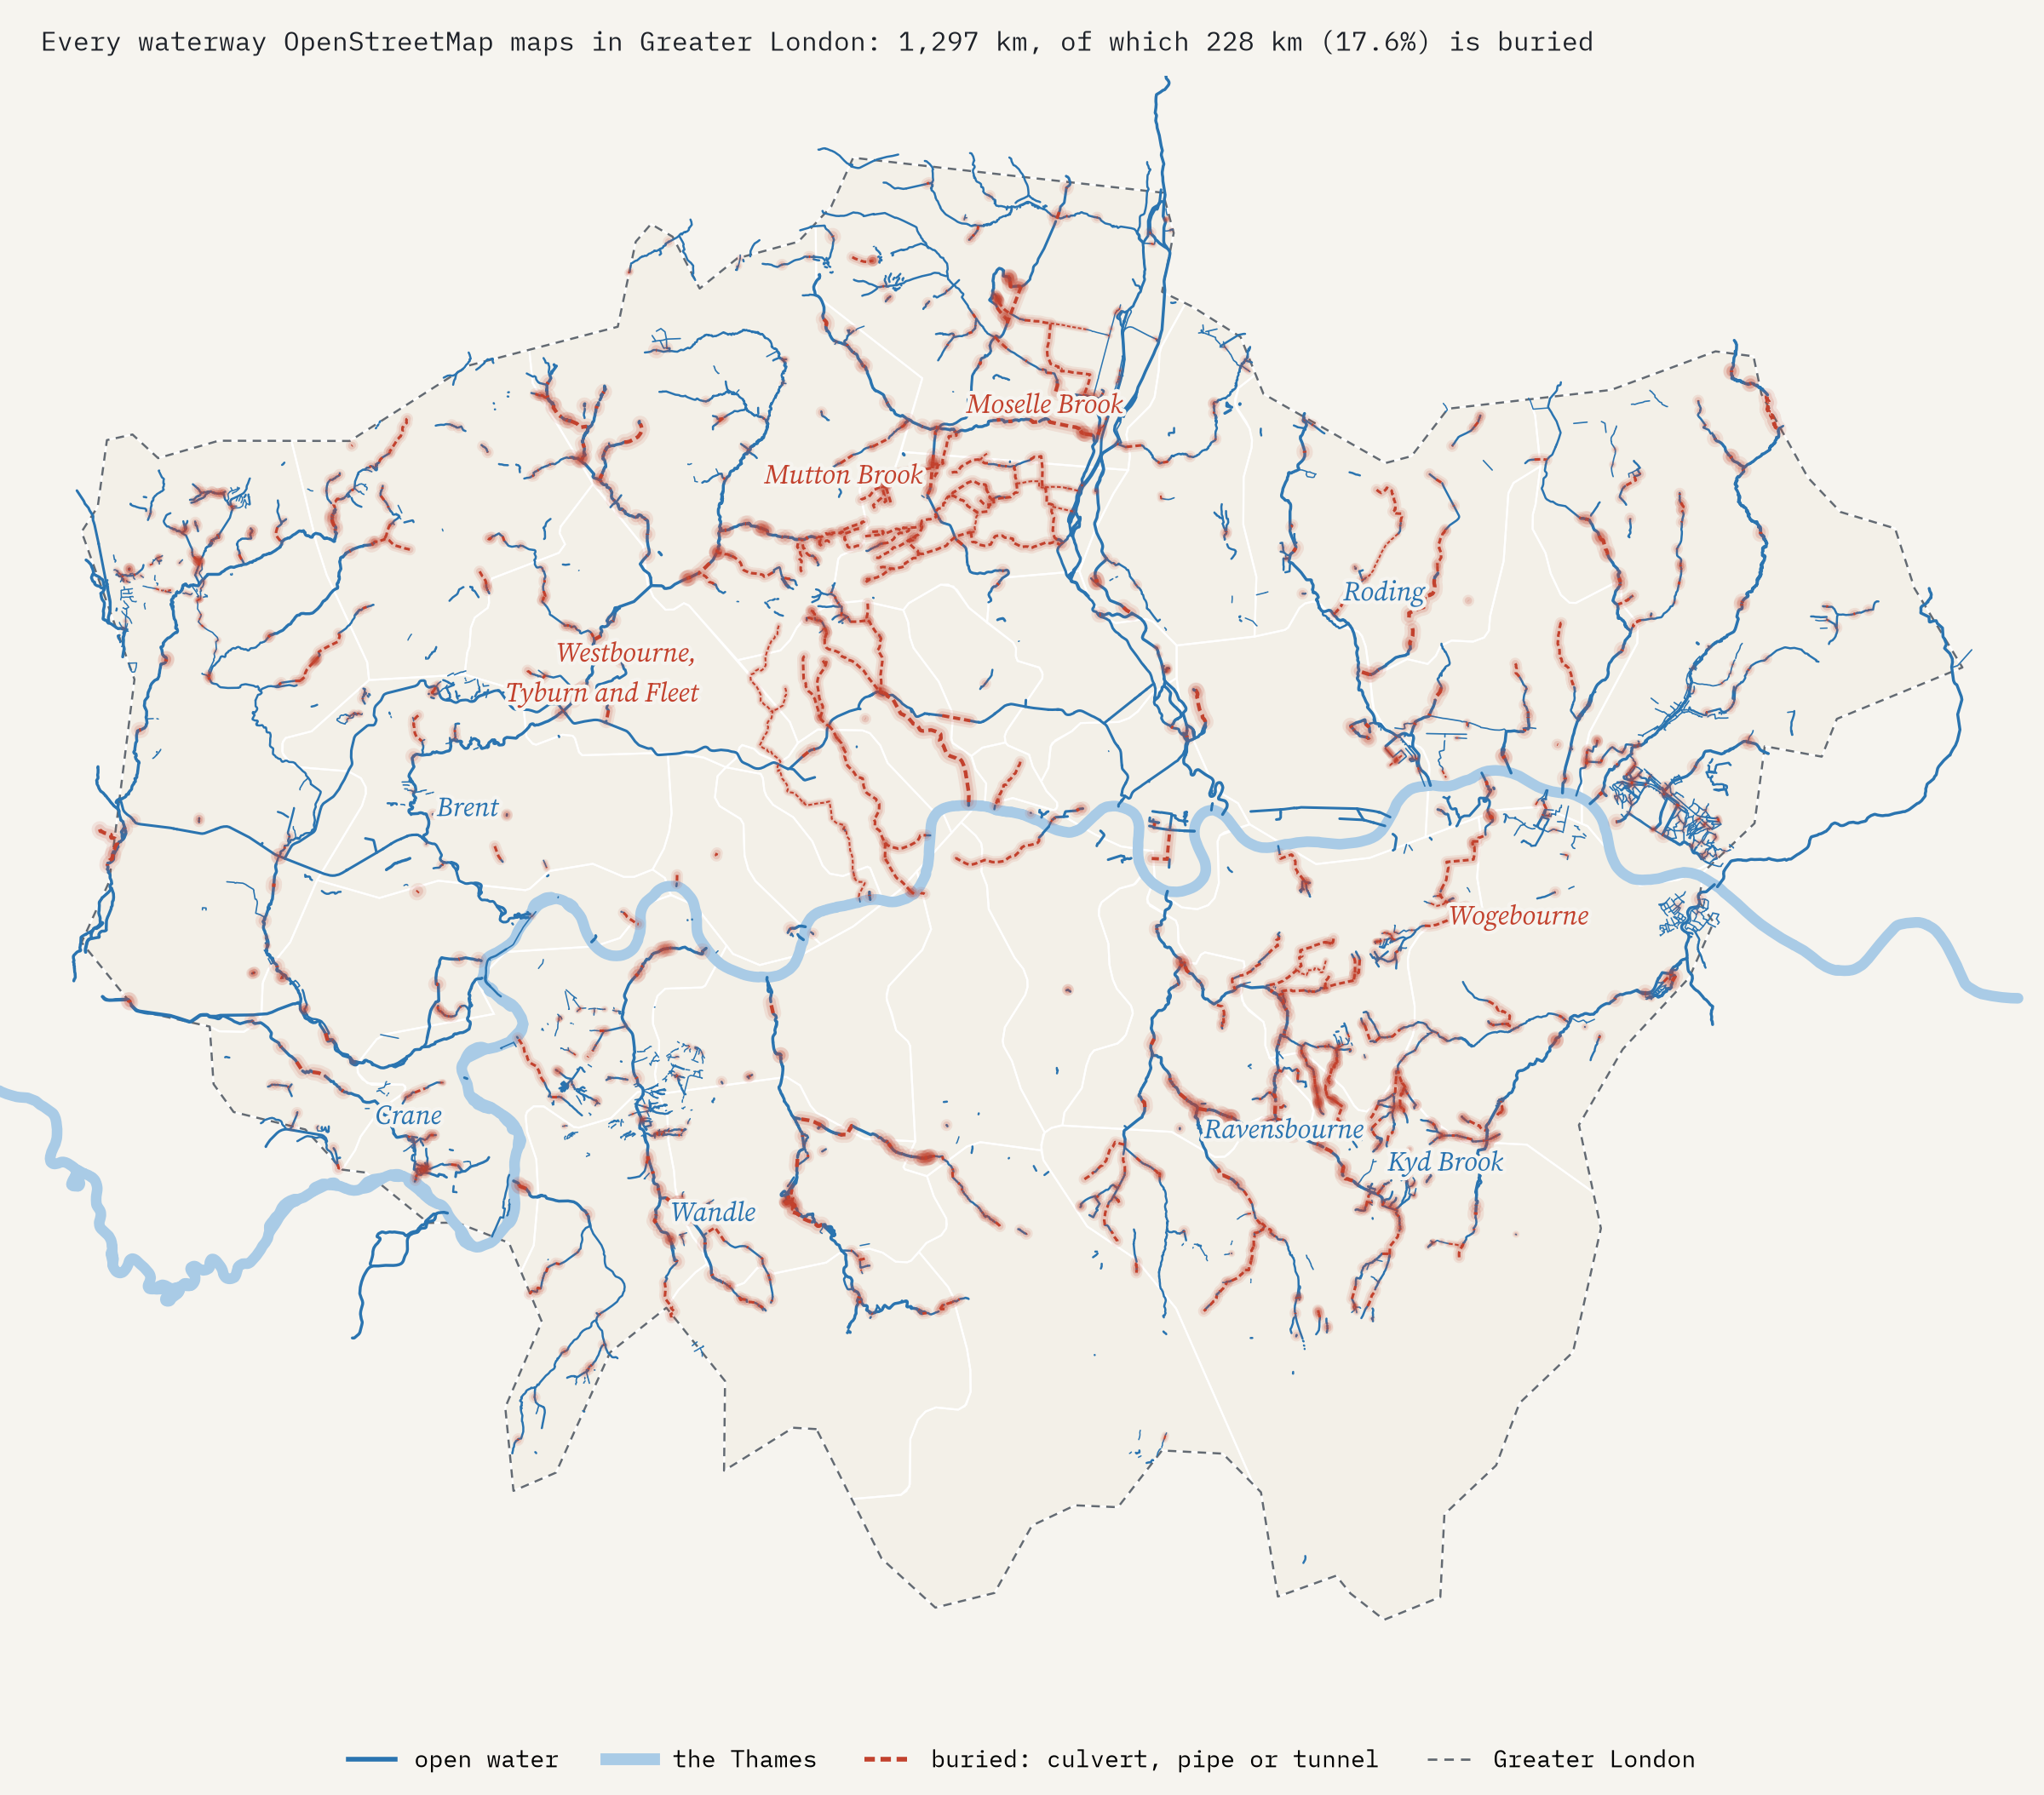
\includegraphics[width=\textwidth]{f_map.png}
\caption{Every waterway mapped in OpenStreetMap inside Greater London: open (blue), buried (red, dashed) and the Thames.}\label{fig:map}\end{figure}

\begin{figure}[tbp]\centering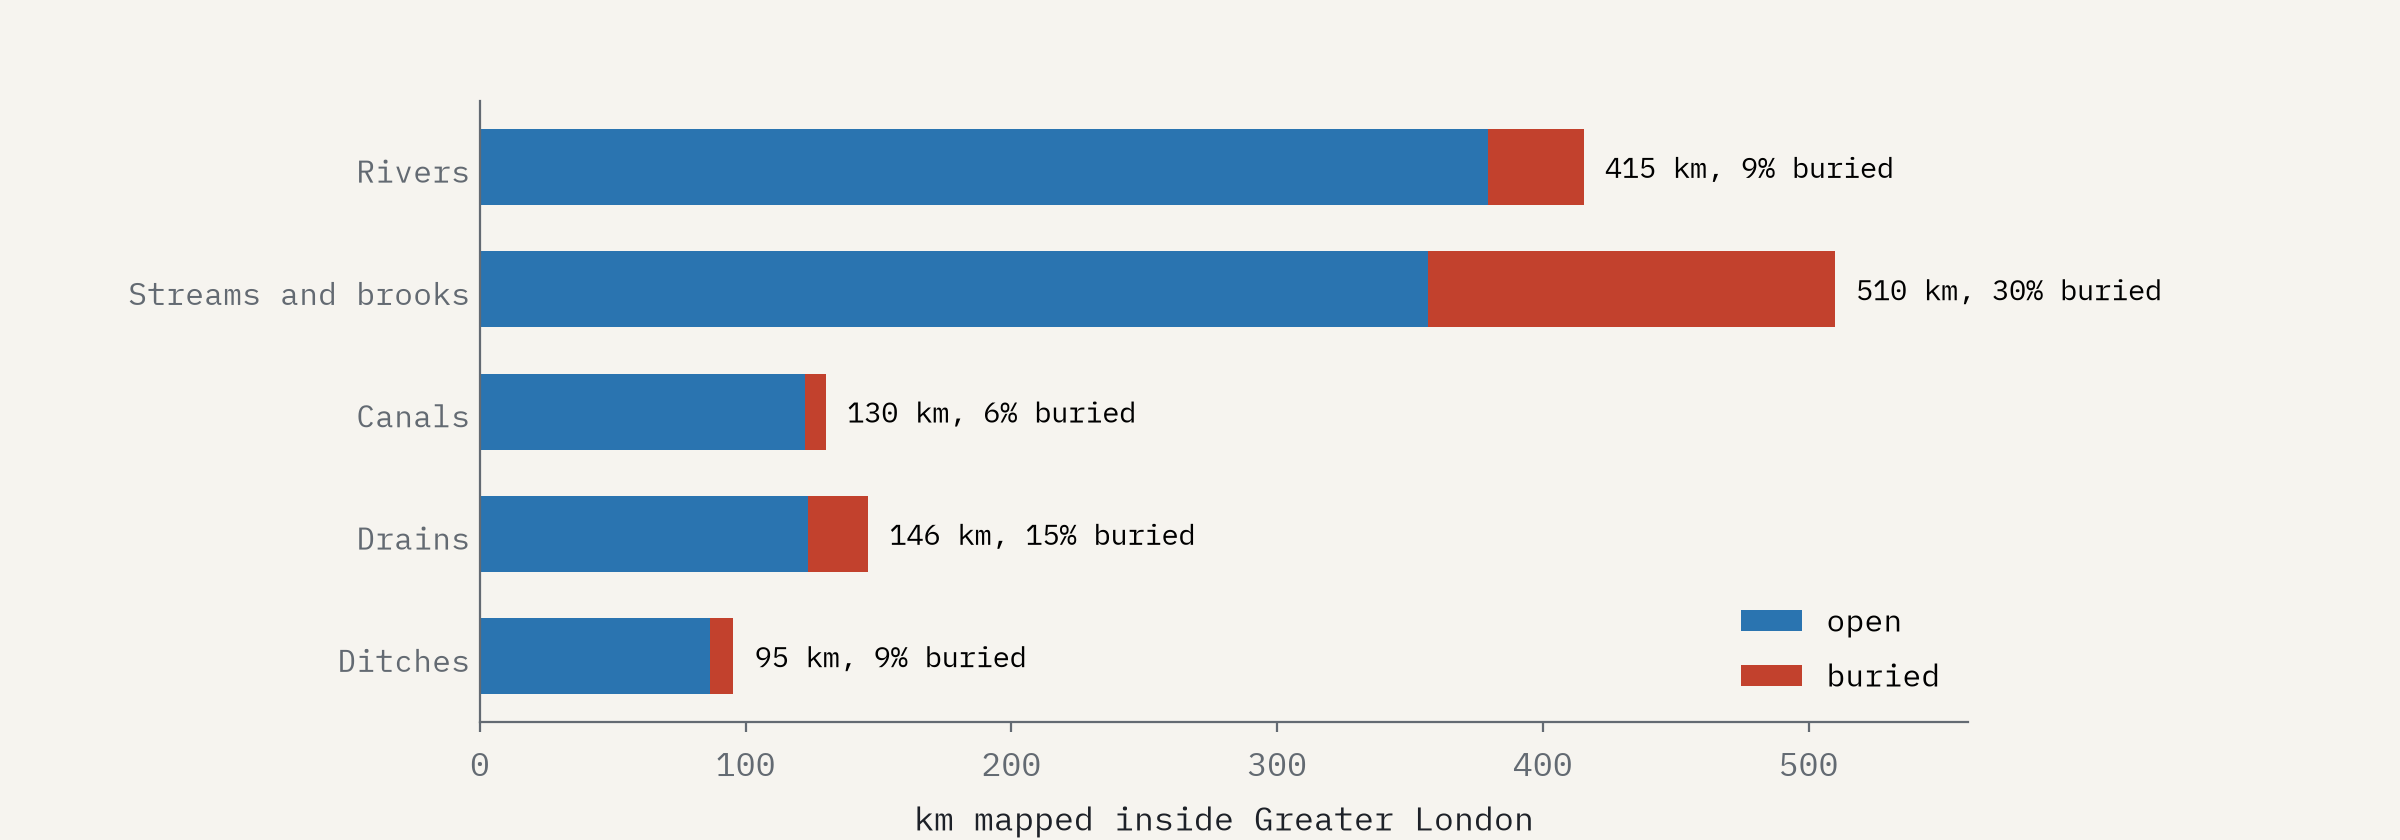
\includegraphics[width=\textwidth]{f_types.png}
\caption{Open and buried kilometres by waterway type, inside Greater London.}\label{fig:types}\end{figure}

\subsection{The most buried rivers}
Of 79 named waterways with at least 3 km mapped, 21 are more than half buried, 4 are buried for all or almost all of their length and 8 have no buried length at all (Table~\ref{tab:rank}, Figure~\ref{fig:rank}). The Tyburn is buried for all 12.1 km mapped, the Westbourne for 99.0\% and the Fleet for 92.6\%, its open length being the headwater streams and ponds on Hampstead Heath. By length the Moselle Brook in Tottenham leads, with 15.7 km of culvert. The four longest buried rivers hold 50.9 km, 22.4\% of all buried waterway in London. Several of the most buried are suburban brooks culverted as estates were built: Stonebridge and Cholmeley brooks in Haringey, Saddler's Mill Stream in Enfield, Cran Brook in Redbridge, Lower Kid Brook in Greenwich.

\begin{table}[tbp]\centering\small\caption{The fifteen most buried named waterways with at least 3 km mapped inside Greater London.}\label{tab:rank}\begin{tabular}{llrrr}\toprule Waterway & Main boroughs & km & Buried km & Buried\\\midrule
River Tyburn & Westminster, Camden & 12.1 & 12.1 & 100.0\%\\
Muswell Stream & Haringey, Enfield & 4.2 & 4.2 & 100.0\%\\
Cholmeley Brook & Haringey & 3.3 & 3.3 & 100.0\%\\
Stonebridge Brook & Haringey & 5.2 & 5.2 & 99.6\%\\
River Westbourne & Westminster, Brent & 12.6 & 12.5 & 99.0\%\\
Lower Kid Brook & Greenwich & 3.1 & 2.9 & 94.4\%\\
River Fleet & Camden, Haringey & 11.5 & 10.6 & 92.6\%\\
Moselle Brook & Haringey, Enfield & 17.3 & 15.7 & 90.7\%\\
Saddler's Mill Stream & Enfield & 5.1 & 4.7 & 90.5\%\\
River Neckinger & Southwark, Lambeth & 3.4 & 3.0 & 87.0\%\\
Cran Brook & Redbridge & 5.0 & 4.3 & 86.1\%\\
The Bourne & Bromley & 3.7 & 2.9 & 79.5\%\\
Well Hall Stream & Greenwich & 3.5 & 2.7 & 76.2\%\\
Mutton Brook & Barnet & 9.4 & 6.2 & 66.3\%\\
Wantz Stream & Barking and Dagenham & 3.3 & 2.2 & 65.2\%\\
\bottomrule\end{tabular}\end{table}

\begin{figure}[tbp]\centering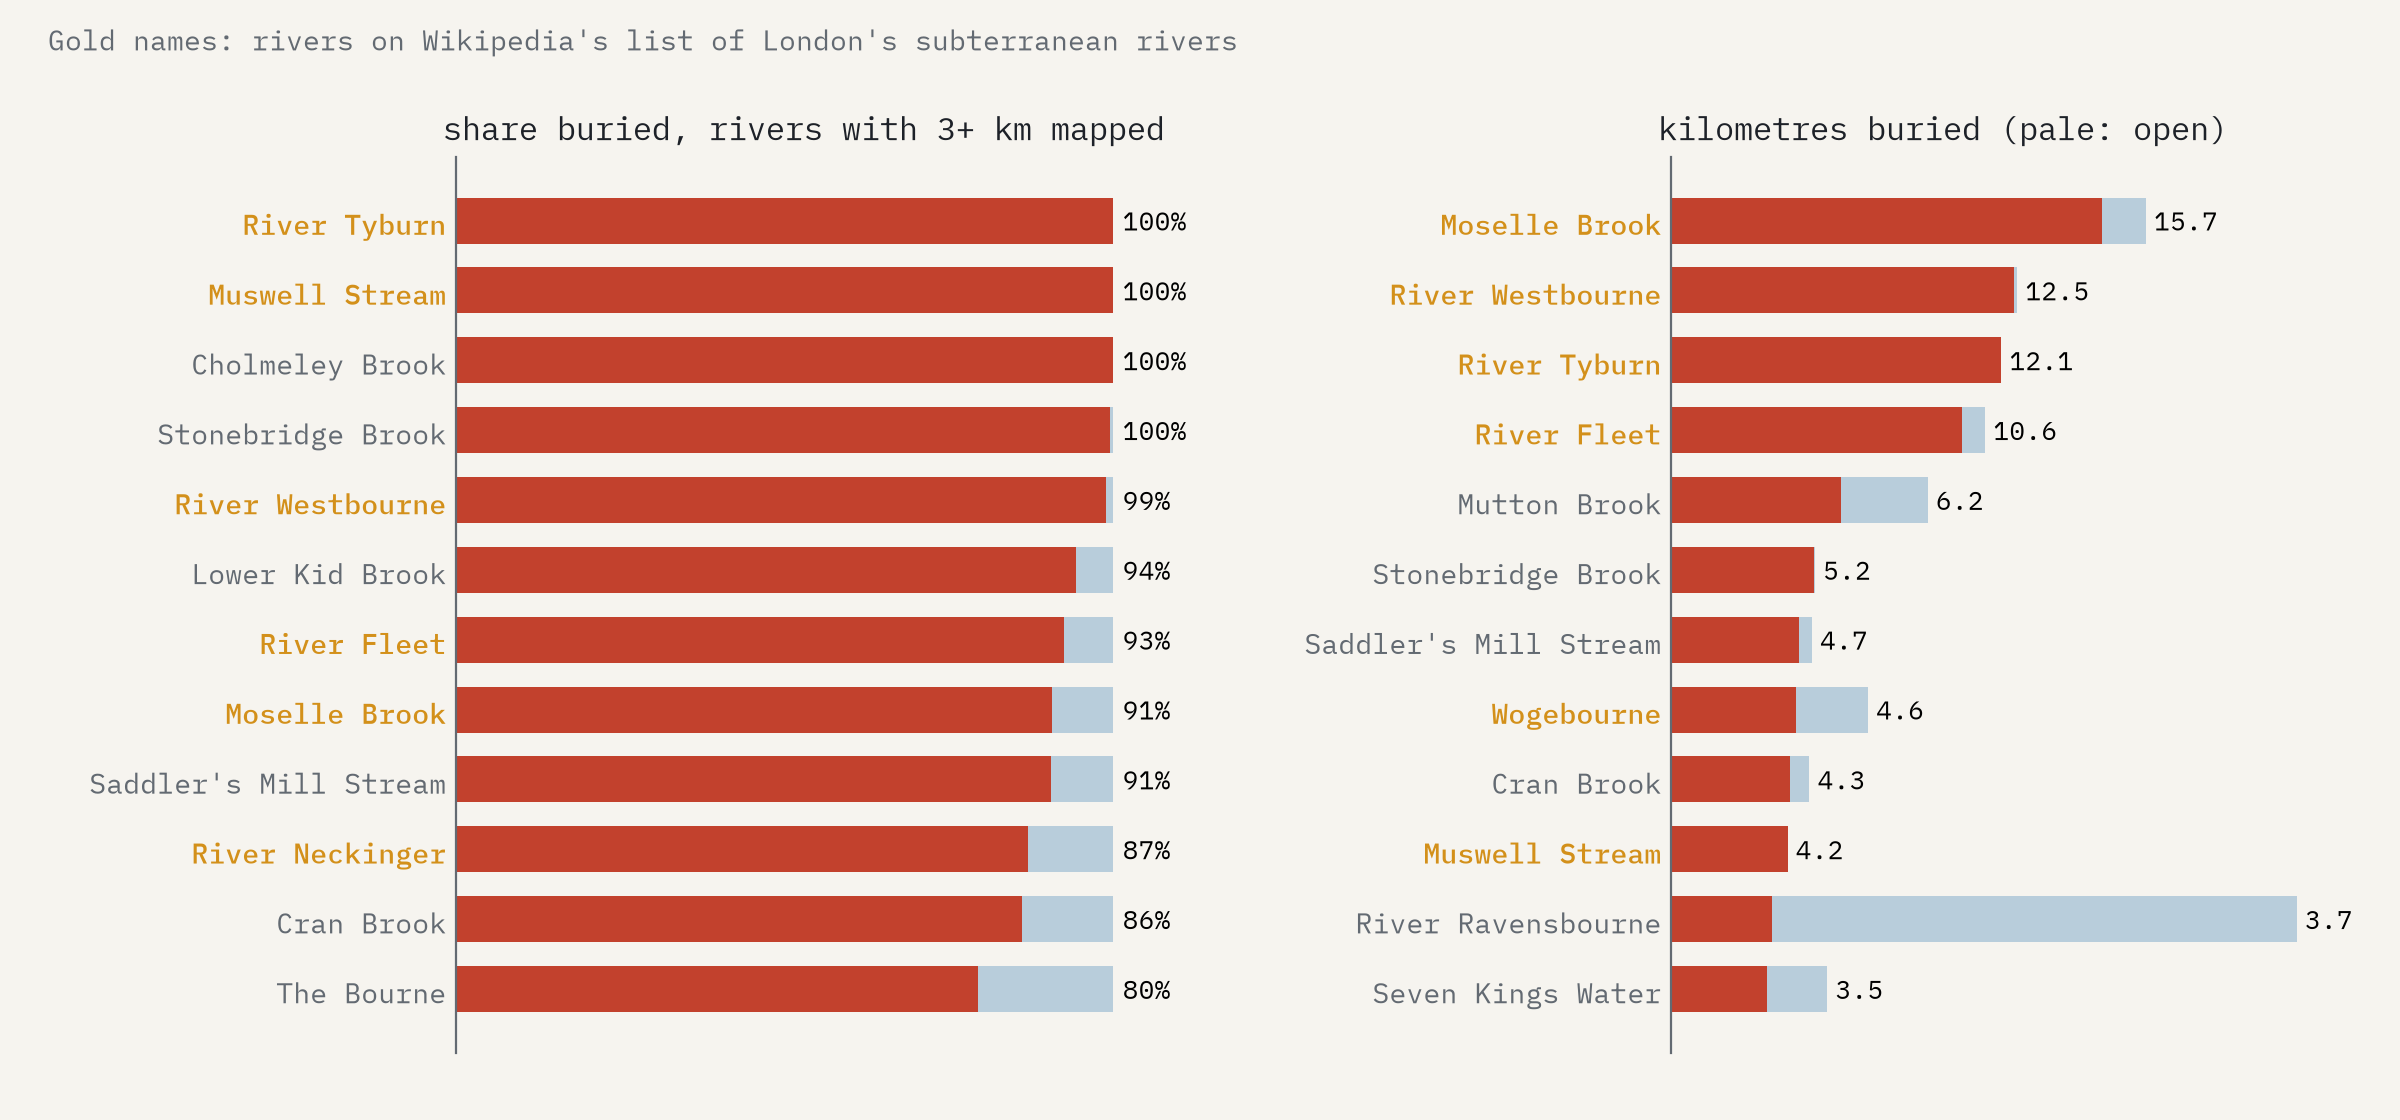
\includegraphics[width=\textwidth]{f_rank.png}
\caption{The most buried named waterways with at least 3 km mapped, by share (left) and by buried length (right). Gold: rivers on Wikipedia's list of subterranean rivers.}\label{fig:rank}\end{figure}

\subsection{The lost rivers}
Table~\ref{tab:lost} and Figure~\ref{fig:lost} compare Wikipedia's lost rivers with what OpenStreetMap maps. The twelve that are mapped total 88.3 km, 77.5\% of it buried, and hold 30.0\% of London's buried waterway. The Fleet, Tyburn and Westbourne together are 97.3\% buried. Five, the Hackney Brook, the Peck, Earl's Sluice, Stamford Brook and Falcon Brook, do not appear as waterways at all. The Effra, whose basin Wikipedia puts at around 20 km\textsuperscript{2}, is represented by 0.13 km of culvert, and Counter's Creek only by Chelsea Creek, its open tidal mouth.

Their histories show the sequence of covering. The Fleet became the New Canal, completed in 1680 under Robert Hooke; it was enclosed between Holborn and Ludgate Circus from 1737, covered below Ludgate by 1769, in King's Cross and Camden from 1812, and in its last open section in the 1870s \citep{wikifleet}. The Westbourne was dammed to form the Serpentine in 1730 and stopped feeding it in 1834; its pipe crosses above the platforms of Sloane Square station \citep{wikiwest}. The Tyburn runs in conduits for its whole length, including beneath Buckingham Palace; the King's Scholars' Pond Sewer that succeeded it was built between 1848 and 1856 \citep{wikityb}. The Effra was an open sewer below North Brixton by 1821 and was arched over in 1847 \citep{wikieffra}; the Peck was enclosed in 1823; the Moselle's stretch by Tottenham High Road was covered in 1836, with more culverting from 1906; Stamford Brook's strands were all covered by 1900; and the Hackney Brook was taken into Bazalgette's northern high level sewer in 1860 \citep{wikirivers}.

\begin{table}[tbp]\centering\footnotesize\caption{Lost rivers named by Wikipedia, side of the Thames, the OpenStreetMap names matched to them, km mapped inside Greater London and the buried share.}\label{tab:lost}\begin{tabular}{lcp{6.2cm}rr}\toprule River & Side & OpenStreetMap names & km & Buried\\\midrule
River Fleet & N & River Fleet, The Fleet & 11.47 & 93\%\\
River Tyburn & N & Tyburn & 12.06 & 100\%\\
River Westbourne & N & River Westbourne, Westbourne & 12.64 & 99\%\\
River Effra & S & Effra & 0.13 & 100\%\\
Walbrook & N & Walbrook & 1.85 & 94\%\\
River Neckinger & S & River Neckinger & 3.42 & 87\%\\
Counter's Creek & N & Chelsea Creek & 0.47 & 0\%\\
Hackney Brook & N & not mapped & 0.00 & \\
Moselle Brook & N & Moselle Brook, River Moselle & 17.34 & 91\%\\
River Peck & S & not mapped & 0.00 & \\
Earl's Sluice & S & not mapped & 0.00 & \\
Stamford Brook & N & not mapped & 0.00 & \\
Muswell Stream & N & Muswell Stream & 4.25 & 100\%\\
Falcon Brook & S & not mapped & 0.00 & \\
Wogebourne & S & Wogebourne & 7.19 & 63\%\\
River Graveney & S & Norbury Brook, River Graveney & 8.68 & 30\%\\
River Quaggy & S & River Quaggy & 8.77 & 14\%\\
\bottomrule\end{tabular}\end{table}

\begin{figure}[tbp]\centering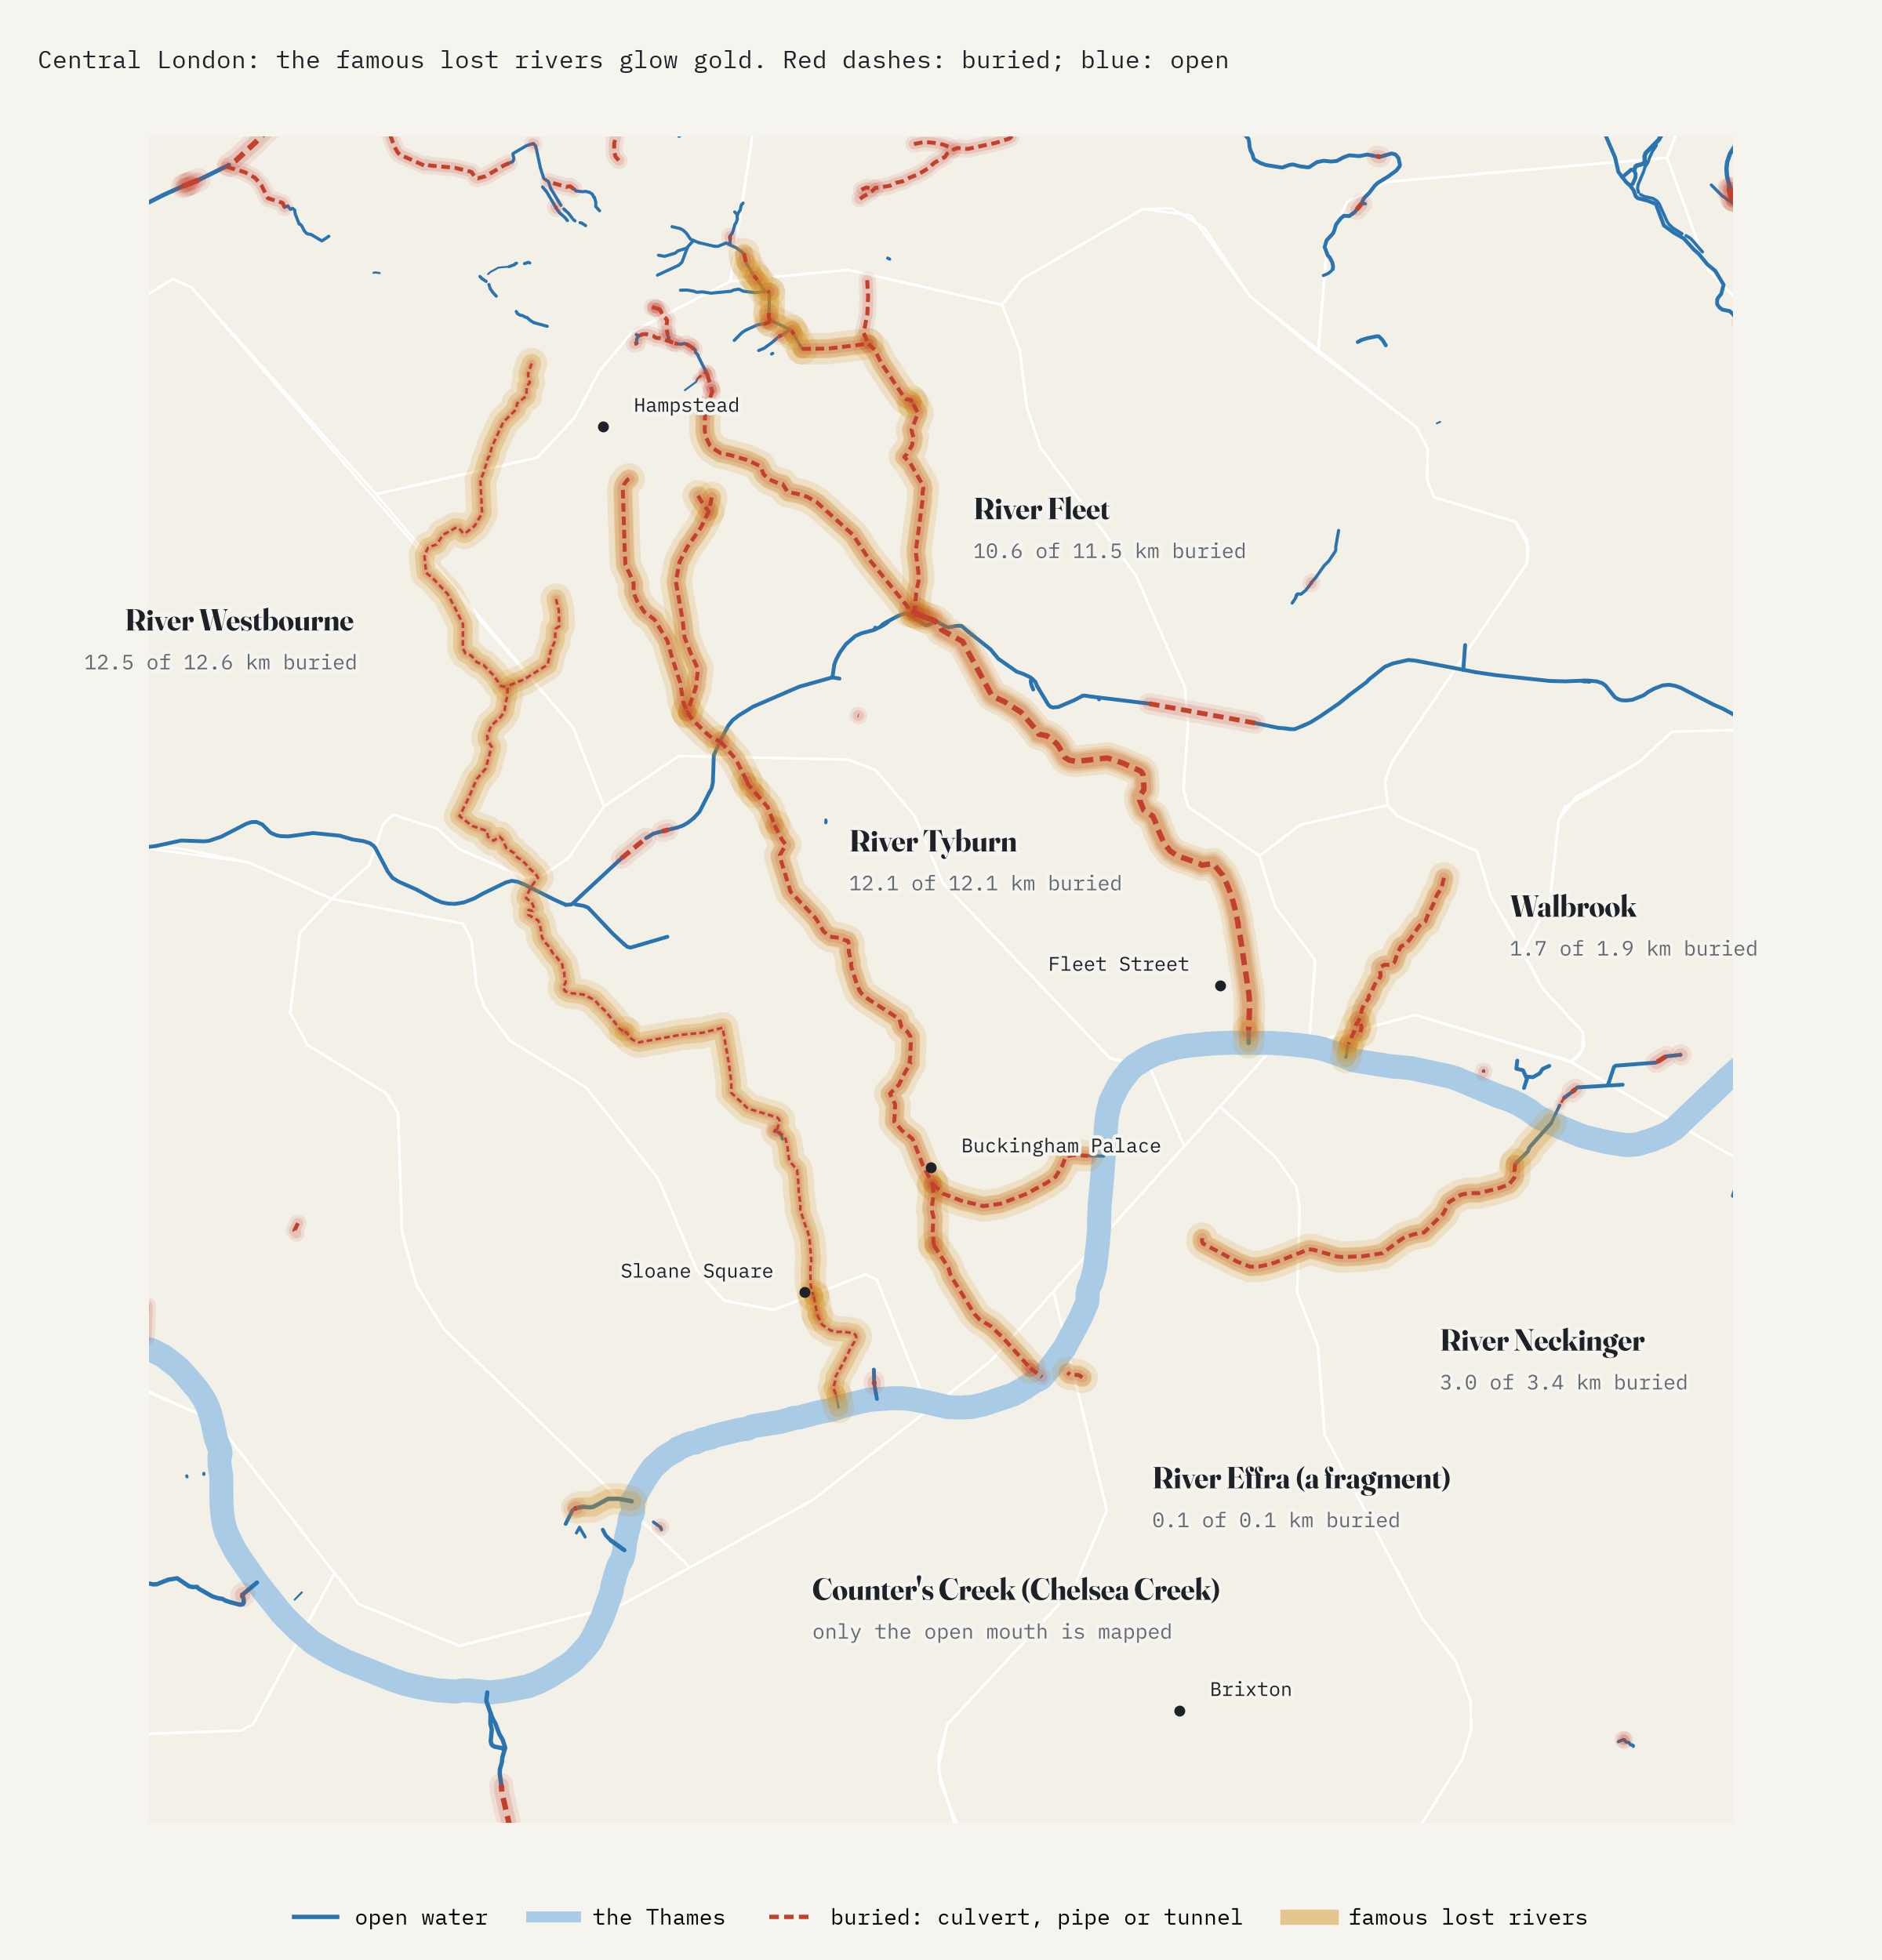
\includegraphics[width=\textwidth]{f_central.png}
\caption{Central London. The famous lost rivers are highlighted in gold; red dashes are buried, blue open.}\label{fig:central}\end{figure}

\begin{figure}[tbp]\centering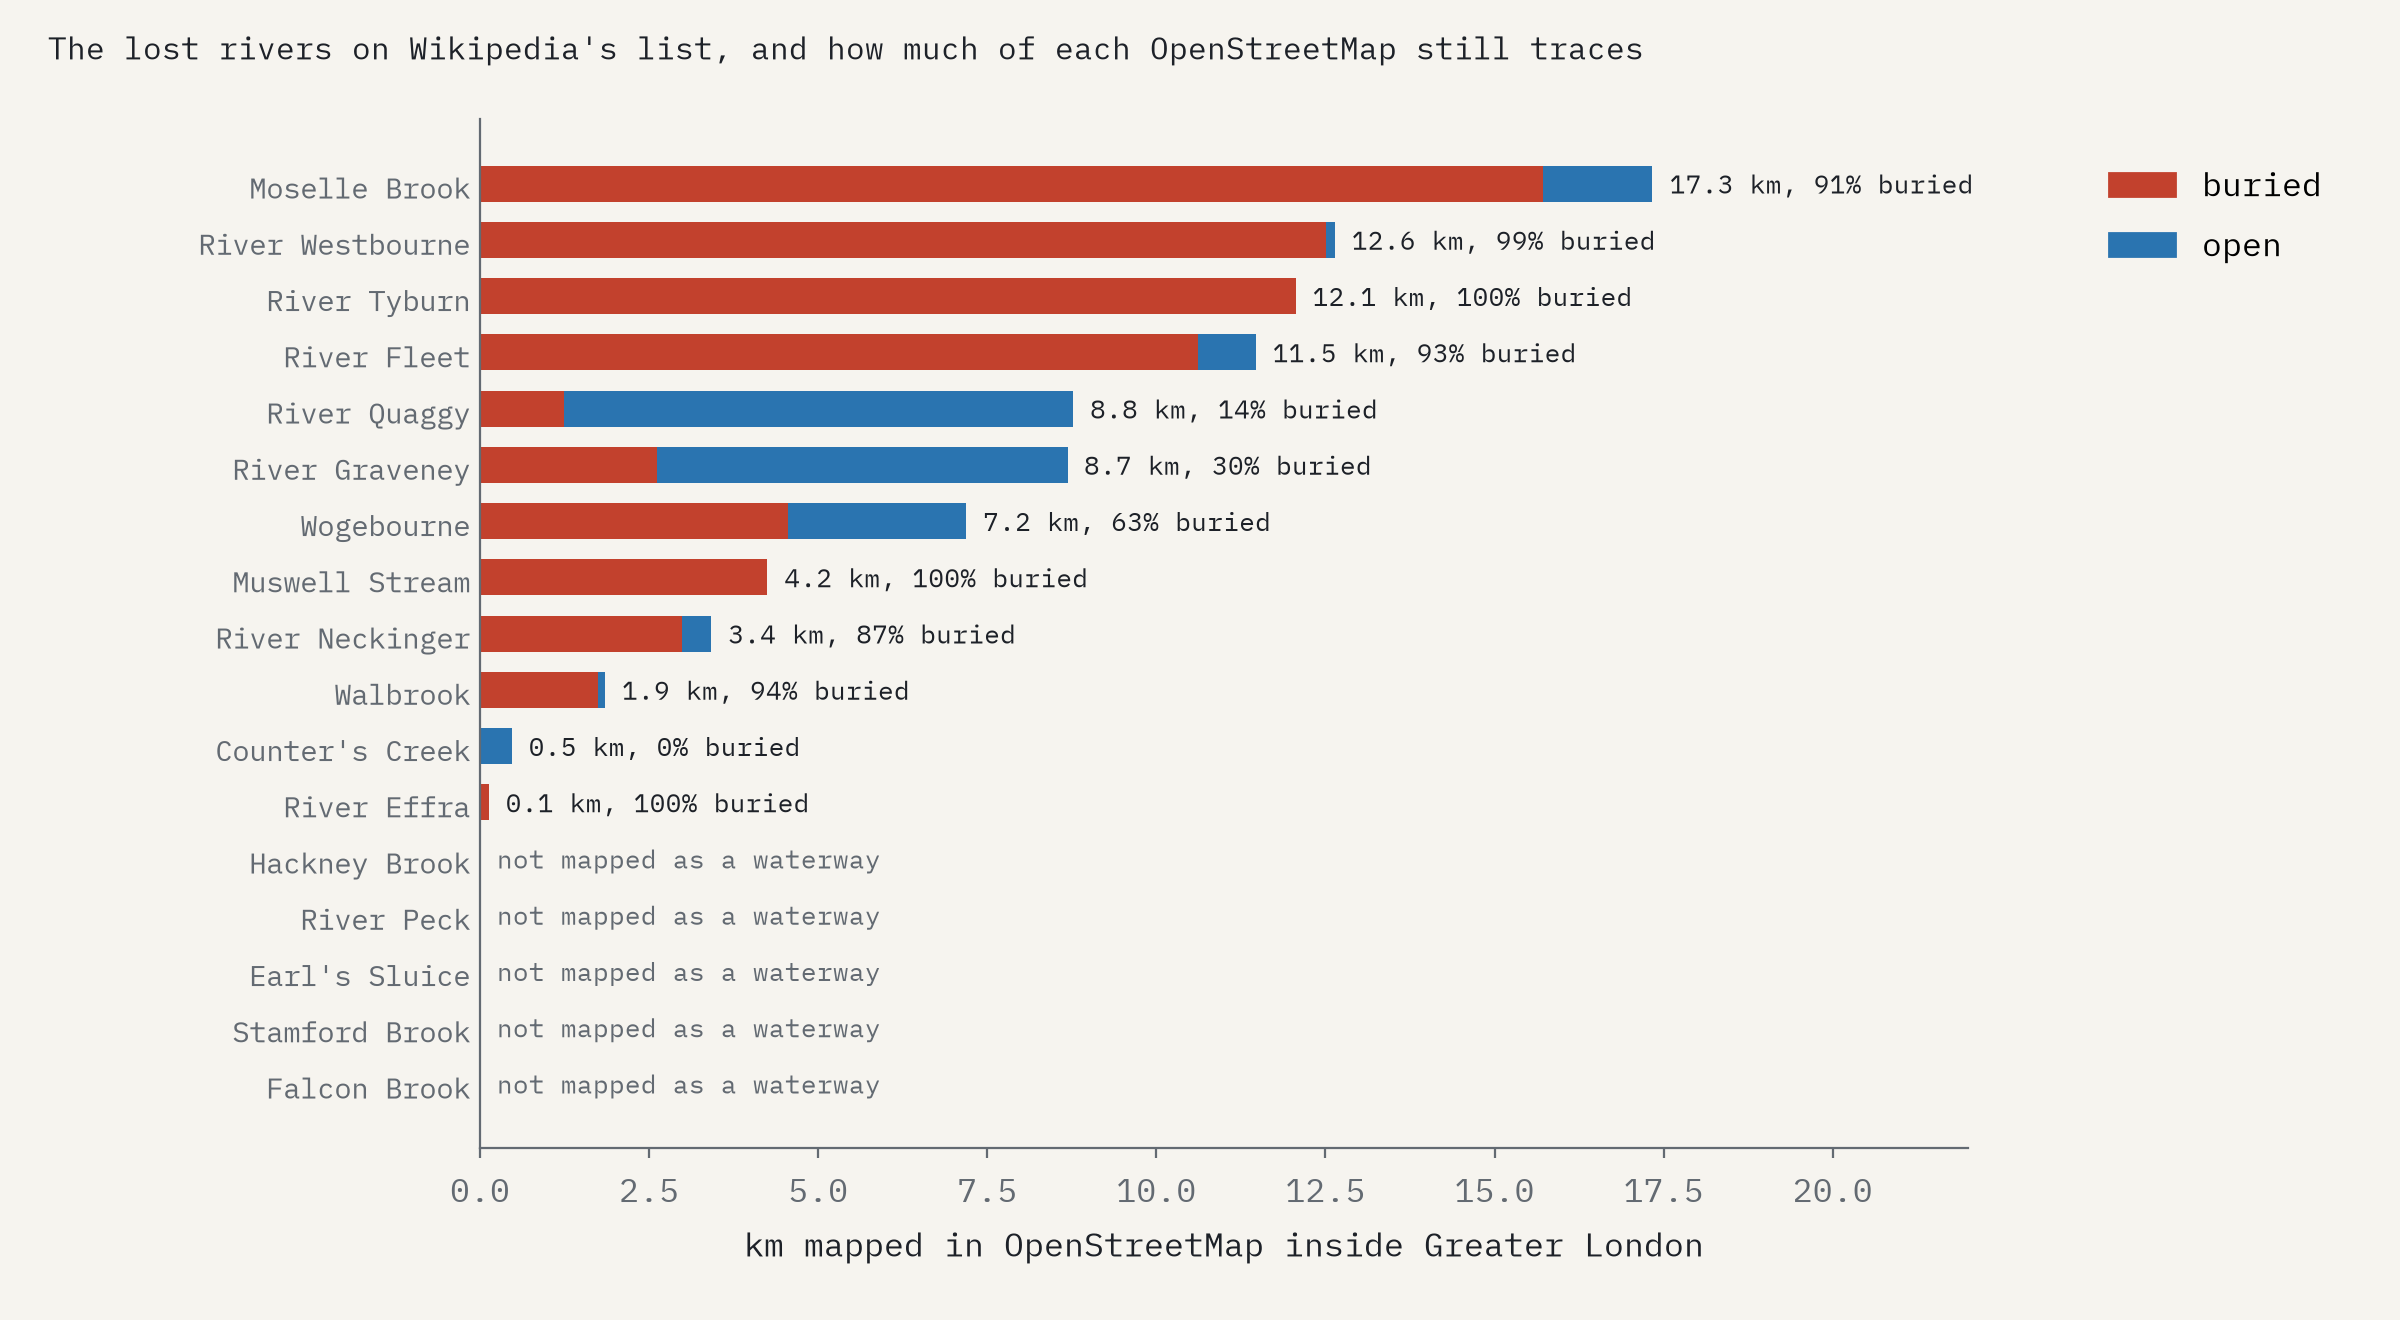
\includegraphics[width=\textwidth]{f_lost.png}
\caption{Wikipedia's lost rivers: length mapped in OpenStreetMap inside Greater London, buried and open.}\label{fig:lost}\end{figure}

\subsection{Boroughs}
Excluding the Thames, inner London's 181 km of mapped waterway is 36.6\% buried; outer London's 1,041 km is 15.5\% buried, a ratio of 2.4. Per unit area the contrast is smaller, 221 against 124 metres of buried waterway per km\textsuperscript{2}, because outer London has more waterway overall (Figure~\ref{fig:boroughs}, Table~\ref{tab:boroughs}). The City (1.6 km mapped) is entirely buried; Westminster (73.8\%) and Camden (72.6\%) follow. Haringey has the most buried length, 34.1 km. Hackney is the least buried borough (1.2\%), an artefact of the Hackney Brook's absence from the map rather than evidence that its rivers survive.

\begin{figure}[tbp]\centering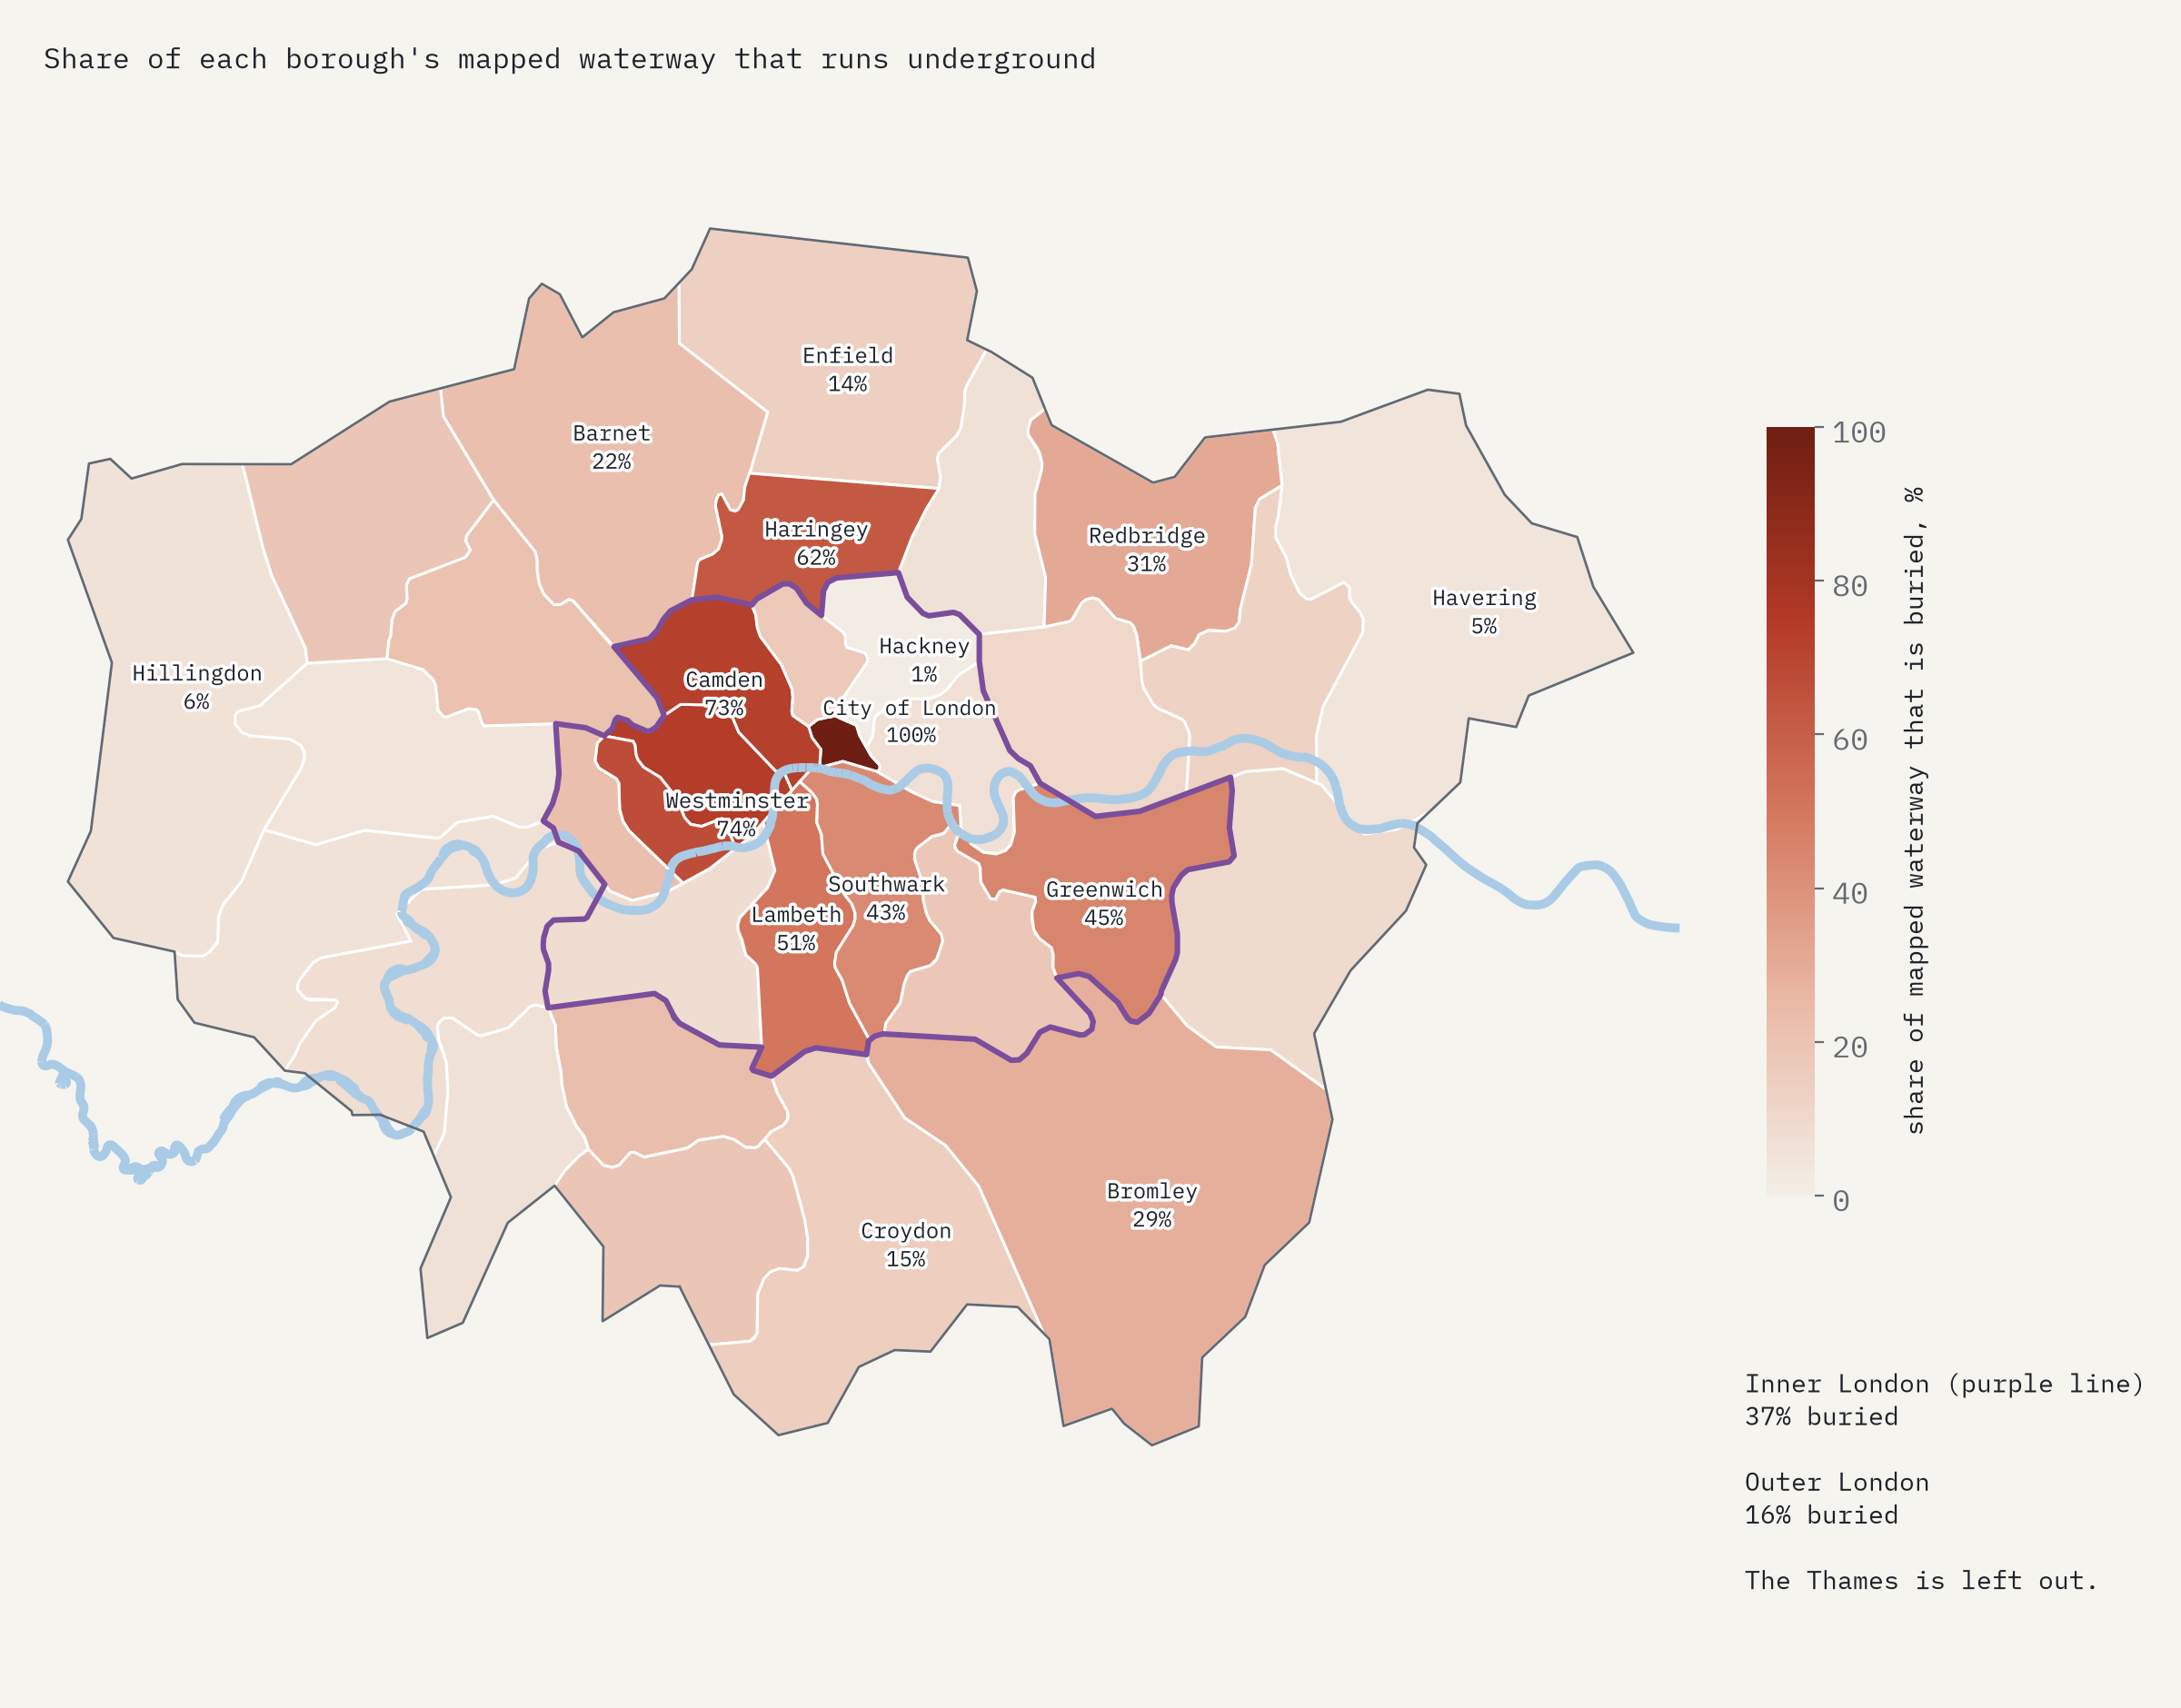
\includegraphics[width=\textwidth]{f_boroughs.png}
\caption{Share of each borough's mapped waterway (excluding the Thames) that is buried. Purple line: inner London.}\label{fig:boroughs}\end{figure}

\begin{longtable}{llrrr}\caption{Boroughs by buried share of mapped waterway, excluding the Thames.}\label{tab:boroughs}\\\toprule Borough & & km & Buried km & Buried\\\midrule\endfirsthead
\toprule Borough & & km & Buried km & Buried\\\midrule\endhead
City of London & inner & 1.6 & 1.6 & 100.0\%\\
Westminster & inner & 17.1 & 12.6 & 73.8\%\\
Camden & inner & 25.9 & 18.8 & 72.6\%\\
Kensington and Chelsea & inner & 1.6 & 1.1 & 67.0\%\\
Haringey & outer & 54.6 & 34.1 & 62.5\%\\
Lambeth & inner & 2.7 & 1.4 & 50.7\%\\
Greenwich & inner & 45.0 & 20.1 & 44.7\%\\
Southwark & inner & 5.6 & 2.4 & 43.0\%\\
Redbridge & outer & 29.9 & 9.3 & 31.0\%\\
Bromley & outer & 75.9 & 21.8 & 28.8\%\\
Merton & outer & 29.4 & 6.8 & 23.0\%\\
Barnet & outer & 81.4 & 17.9 & 22.1\%\\
Hammersmith and Fulham & inner & 1.7 & 0.4 & 22.0\%\\
Brent & outer & 28.1 & 6.0 & 21.4\%\\
Harrow & outer & 29.2 & 5.7 & 19.4\%\\
Sutton & outer & 14.4 & 2.8 & 19.1\%\\
Lewisham & inner & 22.7 & 4.2 & 18.7\%\\
Islington & inner & 3.2 & 0.6 & 17.6\%\\
Croydon & outer & 7.6 & 1.2 & 15.3\%\\
Enfield & outer & 113.8 & 16.3 & 14.3\%\\
Barking and Dagenham & outer & 37.1 & 5.0 & 13.4\%\\
Newham & outer & 27.2 & 3.0 & 10.9\%\\
Bexley & outer & 59.8 & 5.7 & 9.6\%\\
Wandsworth & inner & 14.7 & 1.2 & 8.2\%\\
Richmond upon Thames & outer & 55.1 & 4.2 & 7.7\%\\
Tower Hamlets & inner & 23.3 & 1.6 & 7.0\%\\
Waltham Forest & outer & 24.7 & 1.6 & 6.6\%\\
Kingston upon Thames & outer & 42.9 & 2.8 & 6.4\%\\
Hillingdon & outer & 112.5 & 6.3 & 5.6\%\\
Hounslow & outer & 38.4 & 2.1 & 5.6\%\\
Havering & outer & 138.7 & 7.0 & 5.0\%\\
Ealing & outer & 39.8 & 2.0 & 5.0\%\\
Hackney & inner & 15.7 & 0.2 & 1.2\%\\
\bottomrule\end{longtable}

\section{Limitations}
First, OpenStreetMap is volunteered geographic information. Its coverage of buried water is uneven: some lost rivers are drawn in full along their culverts, some in part, and those that have become sewers are often absent, or mapped as pipelines rather than waterways. The buried totals are therefore a lower bound. Second, tagging varies; a culvert drawn without a tunnel or layer tag counts as open, and a short road culvert on an open stream counts as buried. Third, grouping by name joins ways that share a name and separates tributaries that have their own; the Moselle's relief culvert, for instance, is its own group. Fourth, Natural Earth's generalised outlines make borough figures approximate, especially for rivers that follow boundaries. Fifth, the histories are taken from Wikipedia and are only as reliable as its sources; I give no date that the articles do not.

\section{Conclusion}
About one in six kilometres of London's mapped waterway runs underground, and the share is more than twice as high in inner London as in outer. The burying was concentrated in small streams: the big rivers stayed open, while brooks such as the Tyburn, the Westbourne, the Fleet and the Moselle are almost wholly culverted. The open map is a good record of what was covered and is still traced, but it cannot show the rivers that became sewers. Since the London Rivers Action Plan of 2009, and restorations such as the Quaggy at Chinbrook Meadows, completed in 2002, some of what was buried is being brought back to the surface; a map like this one is a baseline against which that can be measured.

\section*{Data and code availability}
The interactive map is at \url{https://maps.tristanhotham.com/buried-rivers/}. Data and code are at \url{https://github.com/Tristan-Hotham/buried-rivers} and archived with this paper at https://doi.org/10.5281/zenodo.23873535. Code is released under the MIT licence; text and figures under CC BY 4.0; the OpenStreetMap derived data under the ODbL 1.0 (\textcopyright{} OpenStreetMap contributors); the river stories derived from Wikipedia under CC BY-SA 4.0.

\section*{AI statement}
I wrote the text, with drafting and editing assistance from Claude (Anthropic), which also helped prepare the analysis code. I reviewed and checked all text and results.

\begin{thebibliography}{9}
\bibitem[OpenStreetMap contributors(2026)]{osm} OpenStreetMap contributors (2026) OpenStreetMap, waterways in and around Greater London, via the Overpass API. Open Database Licence 1.0. \url{https://www.openstreetmap.org/copyright}
\bibitem[Natural Earth(2026)]{naturalearth} Natural Earth (2026) Admin 1 states and provinces, 1:10m. Public domain. \url{https://www.naturalearthdata.com/}
\bibitem[Wikipedia(2026a)]{wikisub} Wikipedia contributors (2026) Subterranean rivers of London. CC BY-SA 4.0. \url{https://en.wikipedia.org/wiki/Subterranean_rivers_of_London}
\bibitem[Wikipedia(2026b)]{wikifleet} Wikipedia contributors (2026) River Fleet. CC BY-SA 4.0. \url{https://en.wikipedia.org/wiki/River_Fleet}
\bibitem[Wikipedia(2026c)]{wikityb} Wikipedia contributors (2026) River Tyburn. CC BY-SA 4.0. \url{https://en.wikipedia.org/wiki/River_Tyburn}
\bibitem[Wikipedia(2026d)]{wikiwest} Wikipedia contributors (2026) River Westbourne. CC BY-SA 4.0. \url{https://en.wikipedia.org/wiki/River_Westbourne}
\bibitem[Wikipedia(2026e)]{wikieffra} Wikipedia contributors (2026) River Effra. CC BY-SA 4.0. \url{https://en.wikipedia.org/wiki/River_Effra}
\bibitem[Wikipedia(2026f)]{wikirivers} Wikipedia contributors (2026) Articles on Walbrook, River Neckinger, Counter's Creek, Hackney Brook, Moselle Brook, River Peck, Earl's Sluice, Stamford Brook, Norbury Brook and River Quaggy. CC BY-SA 4.0. \url{https://en.wikipedia.org/}
\end{thebibliography}
\end{document}
